\section{Fourier}

\begin{definition}[Fourier-Transformation]
Für Funktionen $ f \in L_{1}(\R) $ definieren wir mit
\[
  \widehat{f} : \R \rightarrow \C, \qquad
  \widehat{f}(\xi) \coloneqq f^{\wedge}(\xi) \coloneqq 
  \int_{\R} f(t) e^{-i\xi t} \dif t, \quad \xi \in \R
\]
die Fourier-Transformierte von $ f $ und für Folgen $ c \in l_{1}(\Z) $
\[
  \widehat{c} : \Z \rightarrow \C, \qquad
  \widehat{c}(\xi) \coloneqq c^{\wedge}(\xi) \coloneqq 
  \sum_{k \in \Z} c(k) e^{-i\xi t}, \quad \xi \in \R
\]
die Fourier-Transformierte von $ c $.
\end{definition}

\begin{remark}[Fourier-Transformation]\leavevmode
\begin{itemize}
\item Was machen wir hier eigentlich? Schreiben wir einfach mal $ \widehat{f} $ als
\begin{align*}
   \int_{\R} f(t) e^{-i\xi t} \dif t
&= \int_{\R} f(t) (\cos(\xi t) - i\sin(\xi t)) \dif t \\
&= \int_{\R} f(t) \cos(\xi t) - i \int_{\R} f(t) \sin(\xi t) \dif t
\end{align*}
dann sehen wir, dass wir lediglich versuchen, $ f $ auszudrücken als Kombination von sinus- und
cosinus-Termen. Wir schauen einfach, wo $ f $ und der $ \sin $ bzw. $ \cos $ eine große Ähnlichkeit
zueinander haben (an der Stelle wird das Integral dann groß) und finden so heraus, welchen 
\enquote{Anteil} die Frequenz $ \xi $ am Signal $ f $ hat. Dass wir hier die doofe imaginäre 
Einheit $ i $ mit drin haben, liegt halt einfach daran, dass wir die Identität
\[
  e^{ix} = \cos(x) + i \sin(x)
\]
ausgenutzt haben, um die Fouriertransformation besonders elegant zu schreiben. Man hätte auch für
Real- und Imaginärteil zwei gesonderte Fouriertransformationen definieren können. Aber das soll uns
hier nicht weiter stören. Außerdem kann man halt mit einer Exponentialfunktion schöner rechnen 
(z.B. ist die Stammfunktion der Exponentialfunktion wieder die Exponentialfunktion). Das ist 
eigentlich alles, was dahinter steckt. Will man die imaginäre Einheit ganz wegbekommen, geht man 
im diskreten Fall einfach über zur \emph{Diskreten Cosinus-Transformation}.
\item Wichtig: Mit der Fouriertransformation finden wir zwar heraus, welche Frequenzen im Singal 
stecken,
aber wir wissen nicht, an welcher Stelle bzw. zu welchem Zeitpunkt die entsprechende Frequenz 
auftritt! Wir haben keine Lokalität, da wir ja über ganz $ \R $ integrieren. Das ist ein wichtiger 
Unterschied zur \emph{Gabor-Transformation}, wo wir unser einer Fensterfunktion bedienen, um so 
Frequenzen besser lokalisieren zu können $ \smiley $.
\item Warum brachen wir $ L_{1}(\R) $-Funktionen? Wie vorher schon erwähnt, ist das eine 
hinreichende Bedingung, dass $ \widehat{f} $ überhaupt existiert:
\[
  \widehat{f} \leq |\widehat{f}| = \left| \int_{\R} f(t) e^{-i\xi t} \dif t \right|
  \leq \int_{\R} |f(t)| \underbrace{|e^{-i\xi t}|}_{= 1} \dif t = \int_{\R} |f(t)| \dif t < \infty.
\]
Das Argument lässt sich analog auf $ l_{1}(\Z) $-Folgen übertragen.
\end{itemize}
\end{remark}

\begin{definition}[Translations- und Skalierungsoperator] \leavevmode
\begin{enumerate}
\item Der Translationsoperator $ \tau_{y} $ mit $ y \in \R $ angewendet auf eine Funktion $ f $ ist 
definiert als
\[ \tau_{y} \ f \coloneqq f(\bullet + y). \]
\begin{figure}[h]
	\centering
	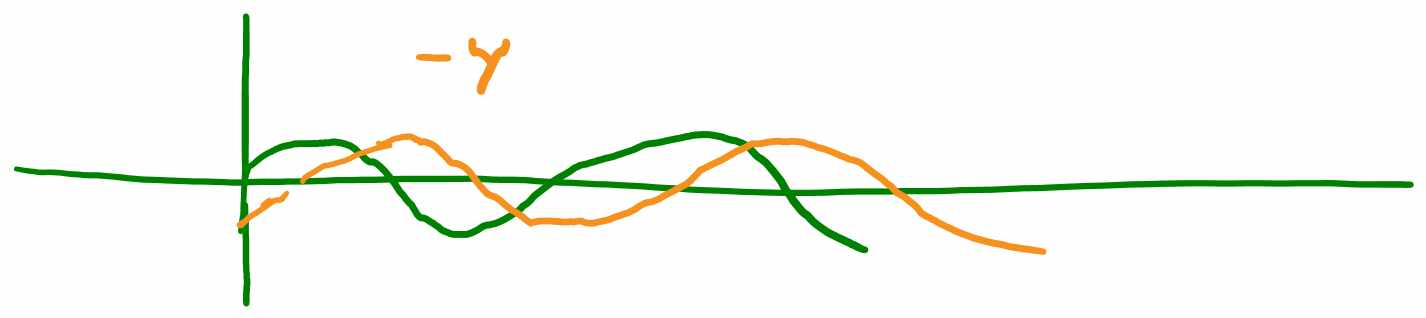
\includegraphics[width=0.5\linewidth]{Bilder/translation}
	\caption{Verschiebung der grün gezeichneten Funktion um $ y $ Einheiten nach rechts führt zur
  	orange dargestellten Funktion.}
	\label{fig:translation}
\end{figure}
\item Der Skalierungsoperator $ \sigma_{h} $ mit $ h \in \R \setminus \{ 0 \} $ angewendet auf eine 
Funktion $ f $ ist definiert als
\[ \sigma_{h} \ f \coloneqq f(h \cdot \bullet). \]
\begin{figure}[ht]
	\centering
	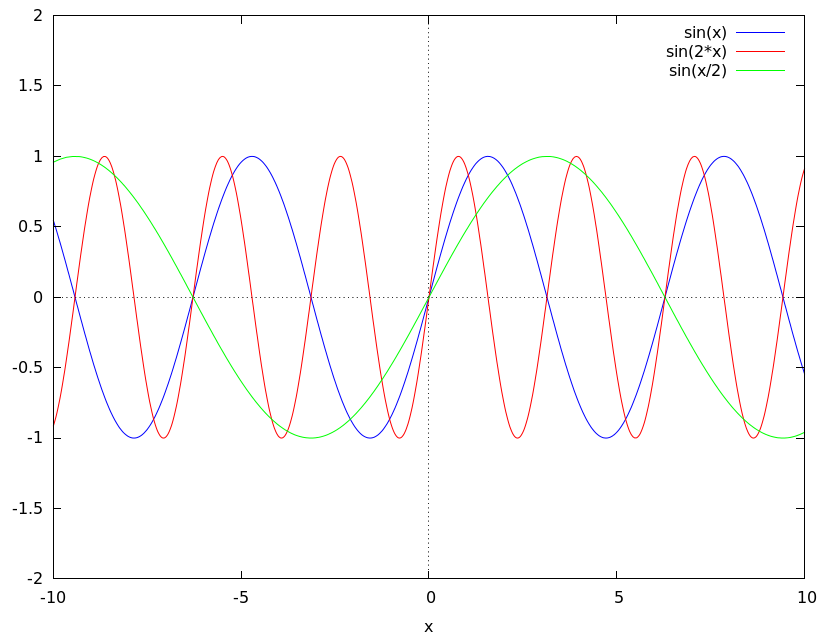
\includegraphics[width=0.5\linewidth]{Bilder/Skalierung.png}
	\caption{Skalierung der sinus-Funktion (blau) mit dem Faktor $ 2 $ führt zu doppelt so schneller
  	Schwingung (roter Graph). Skalierung mit dem Faktor $ 0.5 $ bewirkt halb so schnelle
  	Schwingung (grüner Graph).}
	\label{fig:skalierung}
\end{figure}
\end{enumerate}
\end{definition}

\begin{remark}[Translations- und Skalierungsoperator] \leavevmode
\begin{enumerate}
\item der Translationsoperator verschiebt eine Funktion auf der $ x $-Achse um $ y $ Einheiten nach 
links oder rechts:
\par
\begin{center}
  \begin{tabular}{rl} \toprule
  Wert von $ y $ & Effekt auf $ f $ \\ \midrule
  $ y > 0 $ & Verschiebung nach \emph{links} \\
  $ y = 0 $ & Keine Verschiebung \\
  $ y < 0 $ & Verschiebung nach \emph{rechts} \\ \bottomrule
  \end{tabular}
\end{center}
\item Der Skalierungsoperator streckt oder staucht eine Funktion um den Faktor $ h $ und kann sie 
sogar an der $ y $-Achse spiegeln:\par
\begin{center}
  \begin{tabular}{rl} \toprule
  Wert von $ h $ & Effekt auf $ f $ \\ \midrule
  $ h > 1 $ & Stachung \\
  $ h = 1 $ & Kein Effekt \\
  $ 0 < h < 1 $ & Streckung \\ \midrule
  $ h = 0 $ & Um Gottes Willen! Das ist pfui-gack. \\ \midrule
  $ -1 < h < 0 $ & Streckung und Spiegelung an der $ y $-Achse \\
  $ h = -1 $ & Nur Spiegelung an der $ y $-Achse \\
  $ h < -1 $ & Stauchung und Spiegelung an der $ y $-Achse \\ \bottomrule
  \end{tabular}
\end{center}
\item Die Definition des Skalierungsoperators ist recht ähnlich zur der des Abtastoperators mit
  Schrittweite $ h $. An dieser Stelle sollte betont werden, dass beide Operatoren nicht miteinander
  zu verwechseln sind! Der Abtastoperator liefert zu einem kontinuierlichen Signal $ f $
  ein diskretes Signal $ S_{h} \ f = (f(h \cdot \bullet))_{h \in \Z} $. Das $ h $ ist hier 
  variabel. Der Skalierungsoperator überführt ein kontinuierliches Signal $ f $ wieder in ein 
  kontinuierliches Signal $ \sigma_{h} \ f = f(h \cdot \bullet) $, welches eben um den Faktor $ h $ 
  gestreckt bzw.\ gestaucht wurde. $ h $ ist hier ein fester Wert.
\item Translation und Skalierung sind invertierbar, d.h.\ man kann ihre Auswirkungen wieder
rückgängig machen:
\[
  \tau_{y} \ (\tau_{-y} \ f) = \tau_{-y} \ (\tau_{y} \ f) = f \quad \text{und} \quad
  \sigma_{h} \ (\sigma_{1/h} \ f) = \sigma_{1/h} \ (\sigma_{h} \ f) = f.
\]
\end{enumerate}
\end{remark}

\begin{definition}[Faltung]
Seien $ f, g \in L(\R) $ und $ c,d \in l(\Z) $. Dann ist die Faltung zweier Funktionen definiert als
\[
  f * g \coloneqq \int_{\R} f(\bullet - t) \cdot g(t) \dif t \in L(\R)
\]
und die Faltung zweier Folgen als
\[
  c * d \coloneqq \sum_{k \in \Z} c(\bullet - k) \cdot d(k) \in l(\Z).
\]
Die Faltung einer Funktion $ f $ mit einer Folge $ c $ ist definiert durch
\[
  c * f \coloneqq f * c \coloneqq \sum_{k \in \Z} f(\bullet - k) \cdot d(k) \in L(\R).
\]
\end{definition}

\begin{remark}[Eigenschaften der Faltung]
Aus der Linearität des Integrals und den Gruppenoperationen auf $ \R $ lassen sich folgende 
Eigenschaften der Faltung für Funktionen oder Folgen $ f, g, h $ herleiten:
\begin{itemize}
\item Kommutativität: $ f * g = g * f $
\item Assoziativität: $ (f * g) * h = f * (g * h) $
\item Distributivität: $ f * (g + h) = f * g + f * h $
\item Skalare Multiplikation: $ a \cdot (f * g) = (a \cdot f) * g = f * (a \cdot g) $, wobei
  $ a \in \C $ eine beliebige Konstante ist.
\end{itemize}
\end{remark}
\begin{remark}[Interpretation der Faltung]
Die Faltung kann aufgefasst werden als Produkt zweier Funktionen oder Folgen, welches wieder eine
Funktion bzw. Folge liefert. Wie kann man sich die Faltung geometrisch vorstellen? Betrachten wir 
als Beispiel zwei Funktionen $ f $ und $ g $ und die Faltung $ f * g $. Was dabei passiert, ist 
Folgendes: Zunächst wird $ f $ durch $ f(\bullet - t) $ \emph{vertikal} gespiegelt. Wir halten 
anschließend die Funktion $ g $ fest und lassen $ f $ einmal komplett von ganz links nach 
ganz rechts über die $ x $-Achse wandern. Dort, wo sich $ f $ und $ g $ überlagern und eine große 
\enquote{Gemeinsamkeit} miteinander haben, wird auch das Integral groß. Dort, wo beide Funktionen 
keine große Gemeinsamkeit miteinander haben, wird das Integral klein. Die Faltung ist also eine 
Methode, um feststellen zu können, wie \emph{lokal} ähnlich (nicht global!) sich zwei Funktionen 
sind.

Je nachdem, welche Funktion man für $ g $ wählt, lassen sich mit der Faltung unterschiedliche 
interessante andere Funktionen erzeugen. Wikipedia meint, dass eine Faltung $ f * g $ einen
\enquote{gewichteten Mittelwert} von $ f $ darstellt, wobei die Gewichtung durch $ g $ vorgegeben 
ist. Diese Argumentation versteht man eigentlich erst, wenn man sich \emph{zyklische Faltungen}
anschaut, wo nicht über ganz $ \R $ integriert wird, sondern über ein Kompaktum. Dann wird das
Integral nämlich noch durch die Länge des Kompaktums dividiert, sodass man tatsächlich eine Art
Durschnitt hat. Und hey, das kommt uns doch jetzt irgendwie von der Definition der $ L_{2}(\R) $-
Funktionen bekannt vor!
\end{remark}

\begin{example}[Faltung]
Falten wir doch einmal die Rechtecksfunktion $ \chi_{[-1,1]} $ mit sich selbst. Man definiert
\[
  \chi_{[-1,1]}(x) = \begin{cases} 1, & x \in [-1,1] \\ 0, & \text{sonst}. \end{cases}
\]
Dann ist
\begin{align*}
   (\chi_{[-1,1]} * \chi_{[-1,1]})(x) 
&= \int_{\R} \chi_{[-1,1]}(x - t) \cdot \chi_{[-1,1]}(t) \dif t
 = \int_{\R} \chi_{[x - 1, x + 1]}(t) \cdot \chi_{[-1,1]}(t) \dif t \\
&= \int_{\R} \chi_{[x - 1, x + 1] \cap [-1,1]}(t) \dif t
 = \int_{[x - 1, x + 1] \cap [-1,1]} 1 \dif t \\
&= \begin{cases}
      \int_{-1}^{x+1} 1 \dif t = 2 + x, & -2 \leq x \leq 0, \\
      \int_{x-1}^{1} 1 \dif t = 2 - x, & 0 < x \leq 2, \\
      0, & \text{sonst},
   \end{cases} \\
&\eqcolon \Delta_{[-2,2]}(x).
\end{align*}
Man erhält also die Dreiecksfunktion auf dem Intervall $ [-2,2] $. Was bedeutet das? Naja, die
$ \Delta_{[-2,2]}(x) $ an der Stelle $ x $ gibt genau die Fläche an, die zwischen den beiden 
Rechtecksfunktionen gerade eingeschlossen wird, wenn man eine Rechtecksfunktion um $ x $ Einheiten
verschiebt. Im Fall von $ x = 0 $ überlappen sich beide Rechtecksfunktionen ganz genau, und deren
Flächeninhalt ist $ 2 $. Dies ist genau der Wert von $ \Delta_{[-2,2]}(2) $! Verschiebt man eine
Rechtecksfunktion um $ 1 $ Einheit nach links oder rechts, dann wird nur noch die Hälfte der
Fläche zwischen beiden Rechtecksfunktionen eingeschlossen, also Flächeninhalt $ 1 $. Und genau das
kommt bei $ \Delta_{[-2,2]}(x) $ heraus, wenn man $ x = 1 $ oder $ x = -1 $ einsetzt.

Die geometrische Interpretation einer Faltung ist also sehr vielfältig und hängt sehr stark von den
beiden Funktionen ab, die miteinander gefaltet werden.\\
Bildlich Dargestellt kann man sich dies so vorstellen:
\begin{figure}[h]
	\centering
	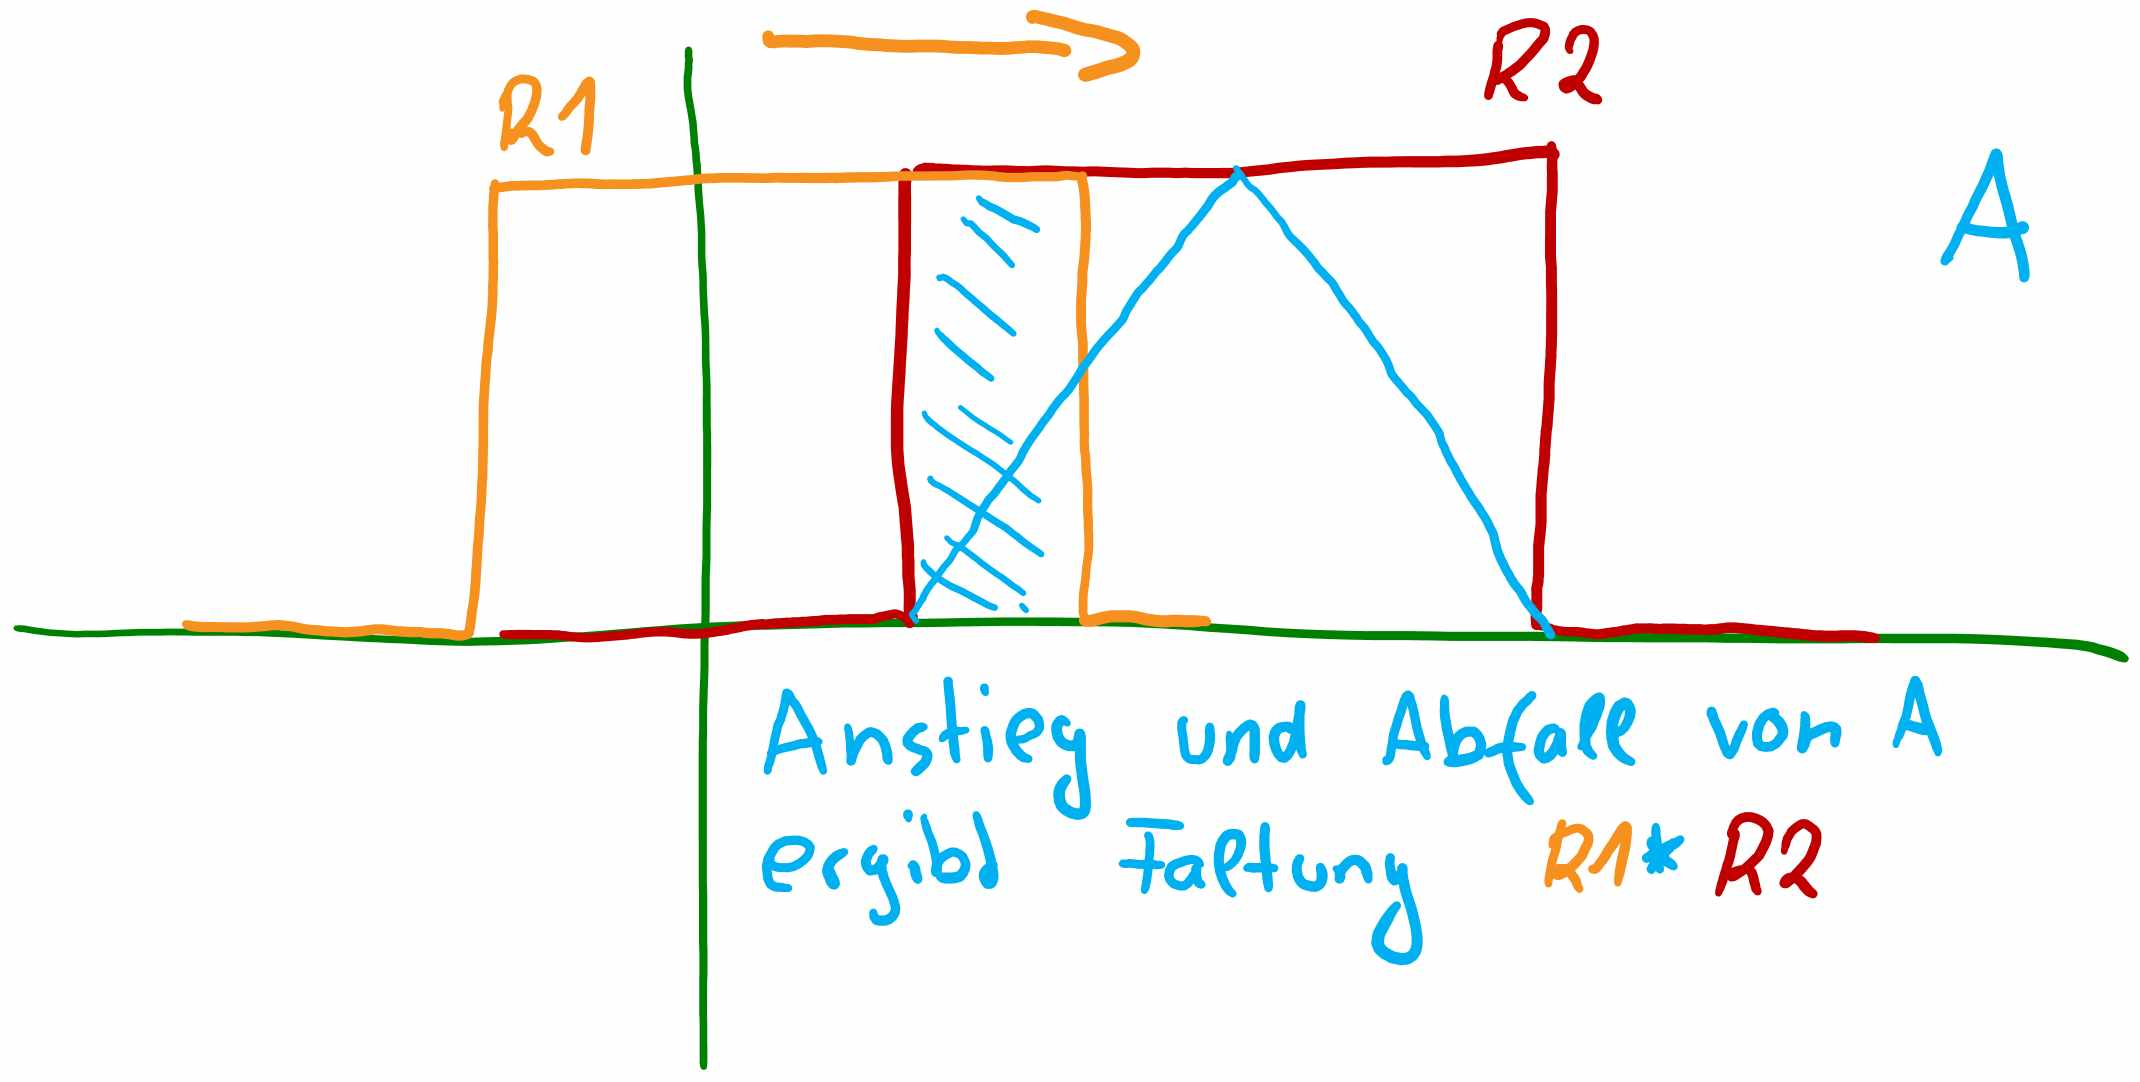
\includegraphics[width=0.7\linewidth]{Bilder/Faltung}
	\caption{Faltung der Rechtecksfunktion (orange und rot) mit sich selbst ergibt die 
  	Dreiecksfunktion (blau).}
	\label{fig:faltung}
\end{figure}
\end{example}

Nun kommen wir zu einem sehr wichtigen Teil der Vorlesung, nämlich zu den Eigenschaften der
Fouriertransformation. Insbesondere wollen wir uns mit deren graphischer Deutung beschäftigen.
Faltungen werden in diesem Kontext auch eine sehr wichtige Rolle spielen, wenn wir die
Fouriertransformierte besonders schnell berechnen wollen.

\begin{remark}[Eigenschaften der Fouriertransformation und deren graphische Deutung] \leavevmode
	 %%Hier könnten wir zu jeder Eigenschaft kurz schreiben was sie bedeuten und falls nötig oder 
	 %%möglich durch Bilder
	%%veranschaulichen
	\begin{enumerate}
  	\item Die Fouriertransformierte ist linear. Dies folgt sofort aus der Linearität des Integrals.
  	Seien also $ f, g \in L_{1}(\R) $ und $ a, b \in \R $. Dann gilt:
    	\[
      	(a \cdot f + b \cdot g)^{\wedge} = a \cdot \widehat{f} + b \cdot \widehat{g}.
    	\]
    
    Bildliche Vorstellung: Multiplizieren wir eine Funktion $ f $ mit einer Konstanten $ a $, so
    ändert sich lediglich die Amplitude von $ f $. Die Frequenzen in der Funktion bleiben gleich,
    es kommen keine neuen Frequenzen hinzu und es fallen keine weg. Der \enquote{Anteil} der bereits
    vorhandenen Frequenzen wird nur anders gewichtet, nämlich mit dem Faktor $ a $ versehen. 
    Deshalb gilt $ (a \cdot f)^{\wedge} = a \cdot \widehat{f} $ (siehe hierfür auch 
    Abbildung~\ref{fig:FT_Linear}, linker Teil).
    
    Was hat es aber mit der Addition zweier Funktionen auf sich? Nun, wenn wir zwei Funktionen 
    addieren, so sollten sich auch die Anteile der Frequenzen addieren. Dies spiegelt sich genau in 
    der Identität $ (f + g)^{\wedge} = \widehat{f} + \widehat{g} $ wider 
    (Abbildung~\ref{fig:FT_Linear}, rechter Teil).
    
    Was passiert, wenn wir $ f = g $ setzen? Dann sollte der Anteil jeder Frequenz doppelt so groß
    sein wie vorher. Und in der Tat: Wir können jetzt entweder sagen 
    $ (f + f)^{\wedge} = \widehat{f} + \widehat{f} = 2 \widehat{f} $ oder
    $ (f + f)^{\wedge} = (2f)^{\wedge} = 2 \widehat{f} $. In beiden Fällen kommt das gleiche raus.
    \begin{figure}[ht]
      \centering
      \begin{minipage}{0.49\linewidth}
        \centering
        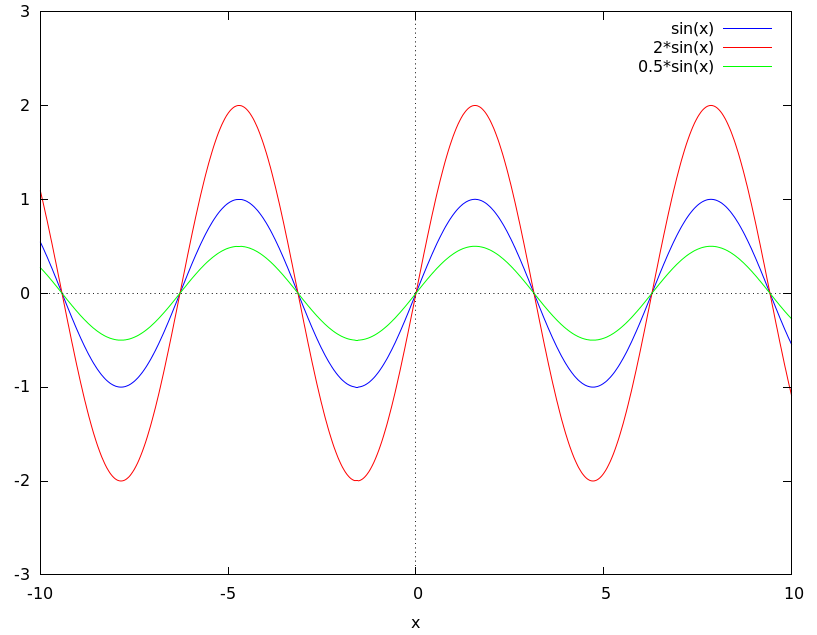
\includegraphics[width=\linewidth]{Bilder/FT_Linear1}
      \end{minipage}
      \begin{minipage}{0.49\linewidth}
        \centering
        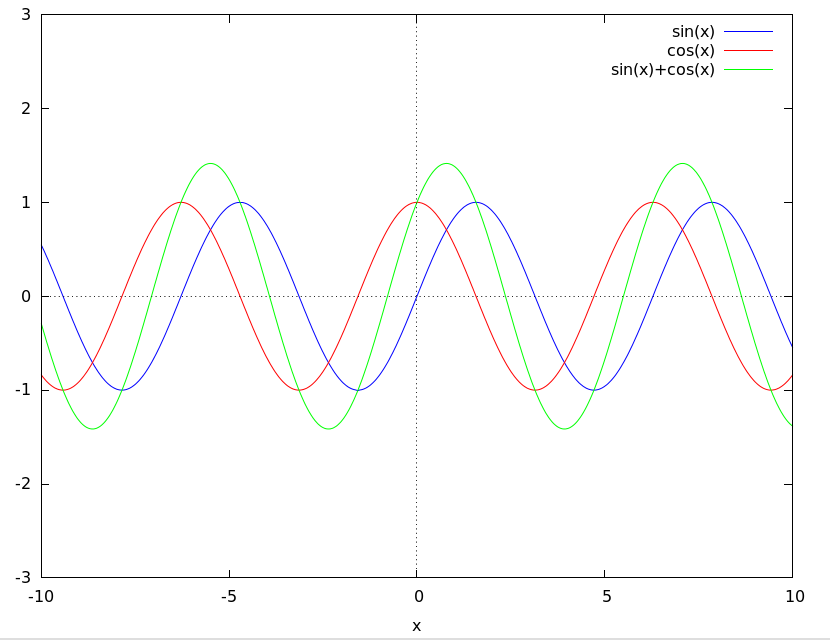
\includegraphics[width=\linewidth]{Bilder/FT_Linear2}
      \end{minipage}
      \caption{Links: Änderung der Amplitude der sinus-Funktion bei gleichbleibender Frequenz.
        Rechts: Bei Addition der sinus- und cosinus-Funktion addieren sich auch die Frequenzen.}
      \label{fig:FT_Linear}
    \end{figure}
		\item Translation (Zeitverschiebung) für $ f \in L_1(\R) $ und $ y \in \R $:
		\[ 
    		(\tau_{y} \ f)^{\wedge}(\xi) 
  		= \left( f(\bullet + y) \right)^{\wedge}(\xi) 
  		= e^{iy\xi}\widehat{f}(\xi), \quad \xi \in \R.
    \]
		Wie bereits oben erwähnt verschiebt eine Translation eine Funktion um den Wert $ y $. 
		Verschiebt man nun die ursprüngliche Funktion des Signal, sollte sich an den Anteilen der 
		Frequenzen $ \xi $ nichts ändern. Wo kommt aber nun dieser seltsame Faktor $ e^{iy\xi} $ her? 
		Dazu müssen wir uns wieder in Erinnerung rufen, dass sich die Fouriertransformation auch so 
		schreiben lässt: $ \int_{\R} f(t) \cos(\xi t) \dif t - i \int_{\R} f(t) \sin(\xi t) \dif t $.\\
		$ \rightarrow $ Es gibt einen Imaginärteil und einen Realteil. Durch die Translation ändert 
		sich nur die Aufteilung zwischen diesen zwei Teilen. Der Gesamtanteil bleibt gleich. Diese 
		Umverteilung geschieht durch den Vorfaktor $ e^{iy\xi} $. (Dies bezeichnet man auch als
		\emph{Frequenz-Modulation}).
		
		Betrachten wir $ \widehat{f} $ als Vektor in der komplexen Zahlenebene, so führt der Faktor $ 
		e^{iy\xi} $ lediglich dazu, dass die 
		der Vektor um den Winkel $ y \cdot \xi $ im Uhrzeigersinn gedreht wird. D.h.\ an den Anteilen
		der Frequenzen ändert sich im Absolutbetrag nichts. Schließlich ist ja auch $ |e^{iy\xi}| = 1 $.
		
		Als veranschaulichendes Beispiel diene hier die Rechtecks-Funktion $ \chi_{[-1,1]} $ mit
		ihrer Fouriertransformierten $ 2\sin(x) / x $. Wird die Rechtecks-Funktion um eine Einheit nach 
		links verschoben, so wird die Fouriertransformierte mit dem Vorfaktor $ e^{i\xi} $ versehen,
		also
		\[   (\tau_{1}\chi_{[-1,1]})^{\wedge}(\xi)
  		 = \left( \chi_{[-1,1]}(\bullet + 1) \right)^{\wedge}(\xi)
  		 = \widehat{\chi}_{[-2,0]}(\xi)
  		 = e^{i\xi} \cdot \frac{2 \sin(\xi)}{\xi}.
  	\]
  	Abbildung~\ref{fig:Rechteck12} zeigt die Rechtecksfunktion und die verschobene 
  	Rechtecksfunktion, sowie deren Fouriertransformierte. Wir stellen zunächst fest, dass die
  	Rechtecksfunktion eine vollständig reelle Fouriertransformierte besitzt und die verschobene
  	Rechtecksfunktion eine reell- und komplexwertige Fouriertransformierte. Dies zeigt ganz 
  	deutlich, dass sich die Aufteilung der Frequenzen zwischen sinus und cosinus verschoben hat. Die
  	interessante Frage ist aber nun: Hat sich an den Anteilen der Frequenzen im Ganzen etwas 
  	geändert? Die Antwort liefert Abbildung~\ref{fig:Rechteck34}. Im Absolutbetrag sind nämlich 
  	beide Fouriertransformationen identisch. D.h.\ die Frequenzanteile sind im Ganzen gleich
  	geblieben. Dies hätte man auch schon so sehen können:
  	\[
    	  \left| (\tau_{1}\chi_{[-1,1]})^{\wedge}(\xi) \right|
    	= \left| e^{i\xi} \cdot \widehat{\chi}_{[-1,1]}(\xi) \right|
    	= \left| e^{i\xi} \right| \cdot \left| \widehat{\chi}_{[-1,1]}(\xi) \right|
    	= 1 \cdot \left| \widehat{\chi}_{[-1,1]}(\xi) \right|
    	= \left| \widehat{\chi}_{[-1,1]}(\xi) \right|.
  	\]
  	
  	Also ganz kurz und knapp: Verschiebung im Zeit-/Ortsbereich führt zu Modulation im
  	Frequenzbereich.
  	
  	Übrigens: Der Realteil der Fouriertransformierten ist immer achsensymmetrisch zur $ y $-Achse,
  	weil der cosinus achsensymmetrisch zur $ y $-Achse ist, und der Imaginärteil ist 
  	punktsymmetrisch um den Ursprung, weil der sinus punktsymmetrisch um den Ursprung ist.
    \begin{figure}[ht]
      \centering
      \begin{minipage}{0.49\linewidth}
        \centering
        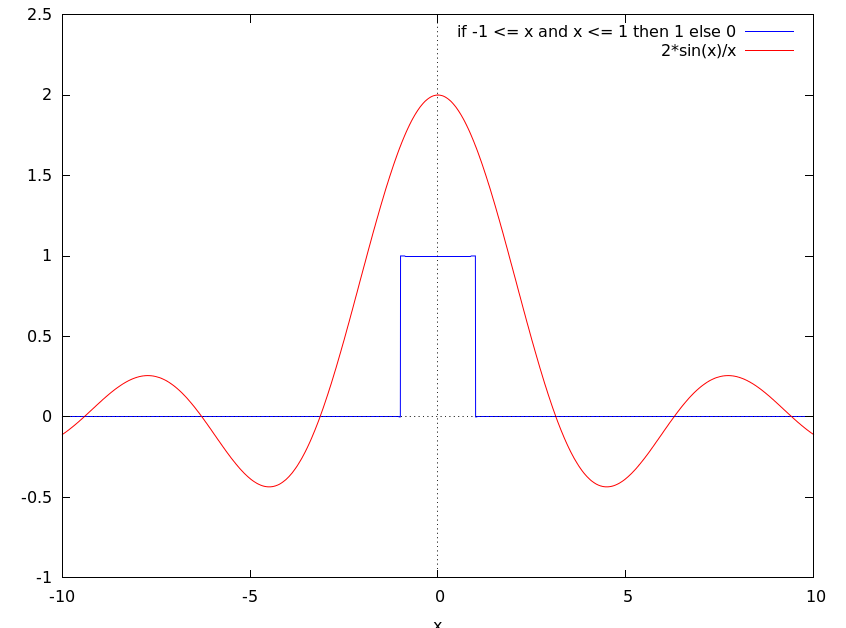
\includegraphics[width=\linewidth]{Bilder/Rechteck1}
      \end{minipage}
      \begin{minipage}{0.49\linewidth}
        \centering
        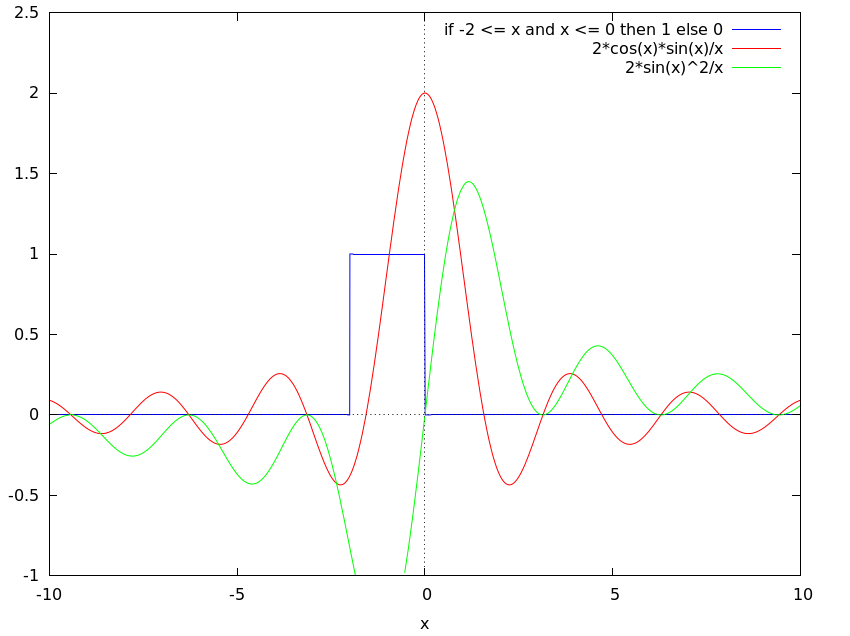
\includegraphics[width=\linewidth]{Bilder/Rechteck2}
      \end{minipage}
      \caption{Links: Rechtecksfunktion und deren Fouriertransformierte. Rechts: Die um $ 1 $
        nach links verschobene Rechtecksfunktion und deren Fouriertransformierte mit Real- und 
        Imaginärteil separat geplottet (Realteil rot, Imaginärteil grün).}
      \label{fig:Rechteck12}
    \end{figure}
    \begin{figure}[ht]
      \centering
      \begin{minipage}{0.49\linewidth}
        \centering
        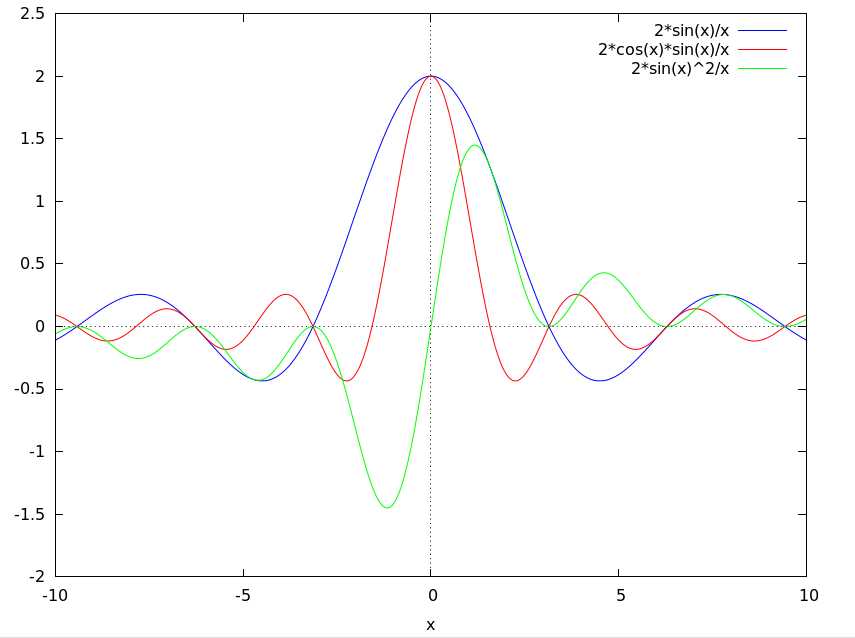
\includegraphics[width=\linewidth]{Bilder/Rechteck3}
      \end{minipage}
      \begin{minipage}{0.49\linewidth}
        \centering
        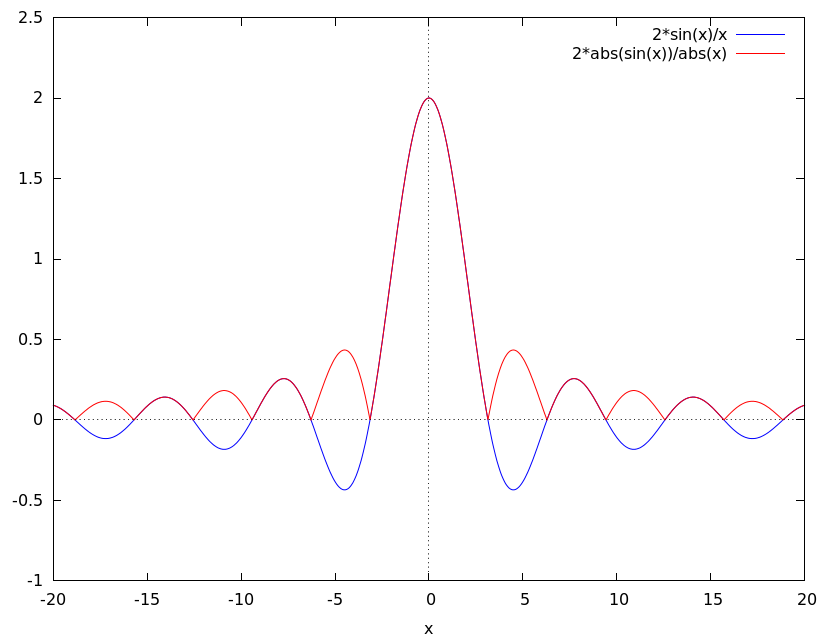
\includegraphics[width=\linewidth]{Bilder/Rechteck4}
      \end{minipage}
      \caption{Links: Fouriertransformierte der Rechtecksfunktion (blau) und der verschobenen
        Rechtecksfunktion (Realteil rot, Imaginärteil grün). Rechts: Fouriertransformation der
        Rechtecksfunktion (blau) und der verschobenen Rechtecksfunktion im Absolutbetrag (rot).}
      \label{fig:Rechteck34}
    \end{figure}
		\item (Zeit-)Skalierung. Sei $ f \in L_{1}(\R) $ und $ h \neq 0 $. Dann gilt
  		\[
      		(\sigma_{h} \ f)^{\wedge}(\xi) 
      	= f(h \cdot \bullet)^{\wedge}(\xi) 
      	= \frac{1}{|h|} \widehat{f} \left( \frac{\xi}{h} \right), \quad \xi \in \R.
  		\]
  	Durch den Skalierungsoperator wird eine Funktion im Zeit-/Ortsbereich in Richtung der $x$-Achse 
  	gestaucht oder gestreckt (anders ausgedrückt: Die Periodenlänge ändert sich). Damit ändern sich
  	auch die im Signal enthaltenen Frequenzen. Beispiel anhand des Sinus: Wird die Periodenlänge 
    halbiert, so verdoppelt sich doch die Frequenz, denn der sinus schwingt jetzt doppelt so 
    schnell. In diesem Kontext ist die Frequenz der Reziprokwert der Periodenlänge.
    
    Können wir diese Analogie auch auf die Fouriertransformation übertragen? Betrachten wir ein
    weiteres Mal die Rechtecksfunktion. Skalieren wir diese mit einem Faktor von $ h = 2 $ und 
    bilden davon die Fouriertransformation, so erhalten wir:
    \[
        (\sigma_{2} \ \chi_{[-1,1]})^{\wedge}(\xi)
      = \frac{1}{2} \widehat{\chi}_{[-1,1]} \left( \frac{\xi}{2} \right) 
      = \frac{2}{\xi} \sin \left( \frac{\xi}{2} \right).
    \]
    Abbildung~\ref{fig:FT_Skalierung} zeigt die eben angesprochenen Funktionen. Das 
    $ \xi /2 $ im Argument von $ (\sigma_{2} \ \chi_{[-1,1]})^{\wedge} $ führt dazu, dass die
    Funktion nur noch halb so schnell schwingt. Durch den Vorfaktor $ 2 / \xi $ verringert sich
    zudem die Amplitude.
    
    \TODO{Eine anschauliche Erklärung hierfür finden!}
    
    Man stellt fest: Für große Werte von $ h $ konzentriert sich die Funktion im Zeitbereich stark 
    um den Ursprung, sie wird gestaucht. Im Frequenzbereich hingegen führt dies dazu, dass die 
    Fouriertransformation gestreckt (auseinander gezogen) und platt gedrückt wird.
    \begin{figure}[ht]
      \centering
      \begin{minipage}{0.49\linewidth}
        \centering
        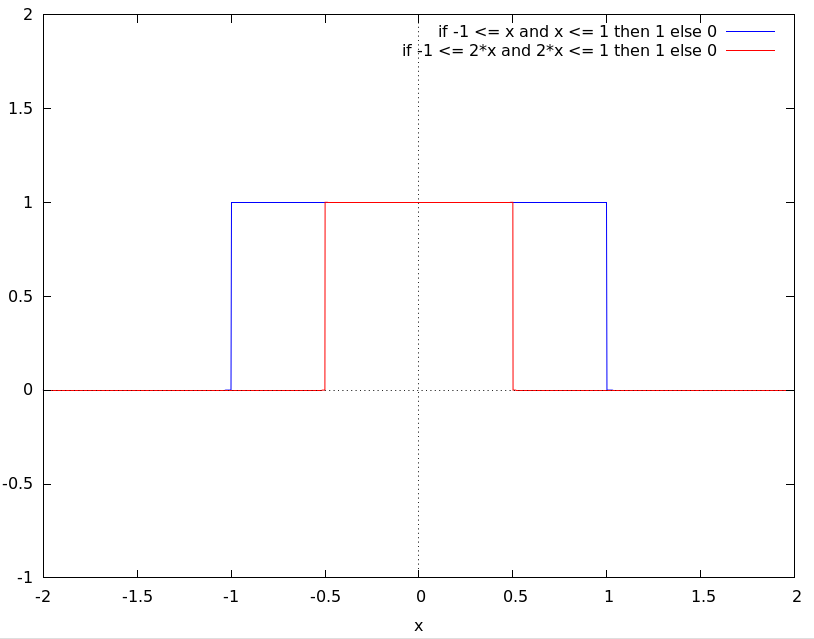
\includegraphics[width=\linewidth]{Bilder/FT_Skalierung_Zeit}
      \end{minipage}
      \begin{minipage}{0.49\linewidth}
        \centering
        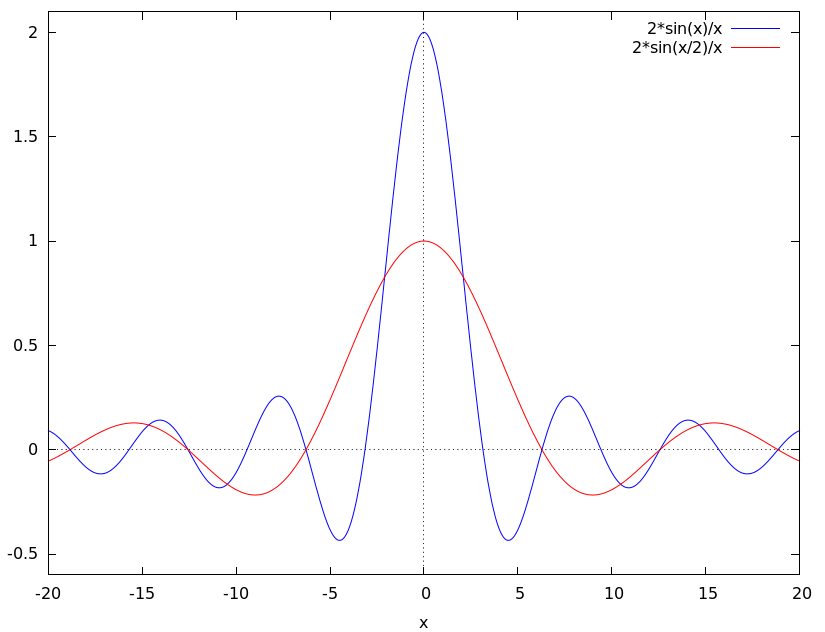
\includegraphics[width=\linewidth]{Bilder/FT_Skalierung_Freq}
      \end{minipage}
      \caption{Links: Rechtecksfunktion (blau) und gestauchte Rechtecksfunktion (rot). Rechts:
        Fouriertransformationen zu den Rechtecksfunktionen (in gleicher Farbe).}
      \label{fig:FT_Skalierung}
    \end{figure}
		\item Faltung
		\item Ableitungseigenschaften
		\item Inverse Fouriertransformation
	\end{enumerate}
\end{remark}